\documentclass[11pt]{amsart}

\usepackage{amsmath,amssymb,amsthm}
\usepackage[margin=1.2in]{geometry}
\usepackage{microtype}
\usepackage{booktabs}
\usepackage{algorithm}
\usepackage{algpseudocode}
\usepackage{tikz}
\usepackage{xcolor}
\usepackage[colorlinks=true,linkcolor=blue!50!black,citecolor=blue!50!black,urlcolor=blue!50!black]{hyperref}

\newtheorem{theorem}{Theorem}[section]
\newtheorem{lemma}[theorem]{Lemma}
\newtheorem{proposition}[theorem]{Proposition}
\newtheorem{conjecture}[theorem]{Conjecture}
\theoremstyle{definition}
\newtheorem{definition}[theorem]{Definition}
\theoremstyle{remark}
\newtheorem{remark}[theorem]{Remark}

\newcommand{\Board}{B}
\newcommand{\Sq}{Q}


\title{The square achievement game on $n \times n$ boards}
\author{Sean Reid}
\date{August 2026}

\begin{document}

\begin{abstract}
Two players alternately claim cells of an $n \times n$ grid; the
first to hold all four corners of an axis-aligned square wins, and a
full board without one is a draw. We give one explicit strategy, two
reflexes over a fixed lookup table with plans confined to a
$6 \times 6$ corner region, that wins every board of size at least
$6$, and with a separate table for $5 \times 5$ we prove that the
first player has a winning strategy if and only if $n \ge 5$, every
smaller board being drawn under optimal play; this answers a question
of Erickson. Boards of size at most $17$ are verified by exhaustive
search, and a simulation theorem with finitely many decidable
hypotheses transports the run at $17$ to every larger board, so the
same strategy is proved to win on every board. The game, the strategy, strategy stealing,
determinacy, and the whole argument are formalized in Lean~4, so the
theorem is machine-checked for all $n$ at once.
\end{abstract}

\maketitle

\section{Introduction}\label{sec:intro}

Two players alternately claim empty cells of an $n \times n$ grid, the
first player moving first. A player wins upon holding all four corners
of a square with horizontal and vertical sides, of any size: the cells
$(r,c)$, $(r,c+s)$, $(r+s,c)$, $(r+s,c+s)$ for some $s \ge 1$. If the
board fills with no player holding such a square, the game is a draw.

Erickson posed the game and asked for the outcome under optimal play
\cite{erickson-pearls, opg}. It is an achievement game in the sense
of Harary \cite{harary}, played in the Maker--Maker convention: both
players pursue the same goal, and a player who loses the race may
still hold out for a draw. The convention itself is older, going back
to the positional games of Hales and Jewett \cite{hales-jewett}; a
recent unified treatment of achievement conventions, with the
strategy-stealing theory in the generality we use, is
\cite{galliot-senizergues}. For the general theory of positional
games see Beck \cite{beck}.

Two boundary results were known. Jenrich \cite{jenrich} reported
computer searches showing that the second player can secure a draw for
$n = 3, 4$ and that the first player can force a win for $n = 5$.
Bacher and Eliahou \cite{bacher-eliahou} proved that every
two-coloring of the $15 \times 15$ grid contains four equal-colored
cells at the corners of an axis-aligned square, and that $15$ is least
with this property. Since no completed game on a board of size $15$ or
more is square-free, strategy stealing gives the first player a win
there. Between these results nothing was published: for
$6 \le n \le 14$ neither a winning strategy nor a drawing strategy was
known \cite{opg}, and no coloring argument can reach this range, since
Bacher and Eliahou also exhibit square-free two-colorings of the
$14 \times 14$ board. Independently and concurrently with the present
work, Adler \cite{adler} announced computer searches for these nine
sizes: a depth-limited negamax with the horizon scored as a draw
returns a first-player win within $13$ plies for each $n$ from $6$ to
$14$; full strategy trees are extracted and certified for $n = 6$ and
$7$, and the remaining sizes are search verdicts under sound pruning
rules. The author notes that the results are unrefereed, and names a
conceptual proof with an explicit strategy as the open direction.

\begin{theorem}\label{thm:main}
In the square achievement game on the $n \times n$ board, the first
player has a winning strategy if and only if $n \ge 5$. For
$n \le 4$ the game is drawn under optimal play: each player can
secure at least a draw.
\end{theorem}

Three things are new here. First, the winning strategy is explicit
and uniform: one lookup table, every plan confined to the
$6 \times 6$ corner region, wins every board of size at least $6$, so
the winning trees for different $n$ are instances of one object
rather than the outputs of separate searches. Second, the proof
covers every $n$ at once: exhaustive verification stops at $17$, and
a simulation theorem carries the checked run to all larger boards, so
the range $n \ge 15$, previously reached only by strategy stealing
from the theorem of Bacher and Eliahou, is covered by the explicit
strategy. Third, the whole argument is machine-checked: the game, the
strategy, the checkers with their soundness theorems, strategy
stealing, determinacy, and the simulation theorem are formalized in
Lean~4, so Theorem~\ref{thm:main} is a single kernel-checked
declaration rather than the output of a program.

Theorem~\ref{thm:main} is proved in three ranges. For $n \le 4$
an exhaustive refutation shows the first player cannot win. For
$5 \le n \le 17$ an explicit strategy, two reflexes (complete a
square when possible, otherwise block an imminent completion) over
fixed lookup tables of forcing plans, is verified by exhaustive
search: the $5 \times 5$ board has its own table, extracted from a
full solution of that game, and a single table with plans confined
to the $6 \times 6$ corner region of the board serves every larger
size. For $n \ge 17$ a simulation theorem transports the checked run
on $\Board_{17}$ to every board at once; its hypotheses are finitely
many decidable properties of the table, each discharged by
evaluation. The proof is therefore constructive on every board and
independent of Proposition~\ref{prop:large}.

Exhaustive searches are only as trustworthy as the programs running
them, and this game is a case in point: the first version of the
search in \cite{jenrich} contained an error and was corrected in a
later revision. We therefore formalize this paper in Lean~4 \cite{lean4},
building on mathlib \cite{mathlib}: the game itself, the checkers
that replay the strategy against every reply sequence, a dual
checker refuting first-player wins on small boards, soundness
theorems for each, and the simulation theorem for arbitrary $n$.
Every search then discharges a statement about the abstract game
rather than about a program. Theorem~\ref{thm:main} is the
declaration \texttt{outcome}, whose proof the kernel checks. The
formal development accompanies this paper as supplementary material.

\section{Definitions and conventions}\label{sec:defs}

\begin{definition}
Cells are pairs of non-negative integers, written $(r, c)$ for row and
column. The board of size $n$ is $\Board_n = \{0, \dots, n-1\}^2$. For
$s \ge 1$, the \emph{square} anchored at $(r, c)$ with side $s$ is the
four-element set
\[
  \Sq(r,c,s) \;=\; \{(r,c),\ (r,c+s),\ (r+s,c),\ (r+s,c+s)\}.
\]
A set $A$ of cells \emph{contains a square} if
$\Sq(r,c,s) \subseteq A$ for some $r, c \ge 0$ and $s \ge 1$.
\end{definition}

The case $s = 1$ is allowed: the smallest winning configuration is a
$2 \times 2$ block of cells. This is the convention of
\cite{jenrich, bacher-eliahou}. Figure~\ref{fig:rules} shows examples
of side $1$ and side $3$; tilted squares do not count.

\begin{figure}[ht]
\centering
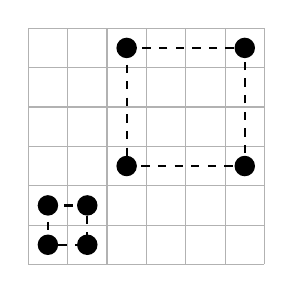
\begin{tikzpicture}[scale=0.5]
  \draw[gray!60] (0,0) grid (6,-6);
  \foreach \r/\c in {4/0, 4/1, 5/0, 5/1, 0/2, 0/5, 3/2, 3/5}
    \fill[black] (\c+0.5,-\r-0.5) circle (0.26);
  \draw[thick,dashed] (0.5,-4.5) rectangle (1.5,-5.5);
  \draw[thick,dashed] (2.5,-0.5) rectangle (5.5,-3.5);
\end{tikzpicture}
\caption{Winning shapes on $\Board_6$: the corners of a $2 \times 2$
block (side $1$) and of a square of side $3$. Only the four corners
must be held; the interior is irrelevant.}
\label{fig:rules}
\end{figure}

A \emph{position} is a pair of disjoint subsets of $\Board_n$, the
stones of the first and the second player. Play alternates, the first
player moving first, each move claiming an empty cell. A player wins
at the first moment their stones contain a square; if the board fills
with neither player holding one, the game is drawn. The game is finite
with perfect information, so exactly one of three statements holds:
the first player can force a win, the second player can force a win,
or both can force at least a draw.

\begin{lemma}[strategy stealing]\label{lem:stealing}
The second player has no winning strategy.
\end{lemma}

\begin{proof}
Suppose the second player had a winning strategy $\tau$. Let the first
player open with an arbitrary move and thereafter follow $\tau$ as if
the extra stone were absent, making a further arbitrary move whenever
$\tau$ selects an occupied cell. The winning condition is monotone in
a player's stone set, so surplus stones never hurt, and the first
player wins; but $\tau$ was assumed to win against all first-player
play, a contradiction. The formal statement is
\texttt{second\_player\_no\_win}; the monotonicity step is the lemma
\texttt{P1CanWin.insert\_left}, whose one subtlety is that the
surplus stone may itself complete a square, ending the game early.
\end{proof}

\begin{proposition}\label{prop:large}
For $n \ge 15$ the first player has a winning strategy.
\end{proposition}

\begin{proof}
A completed game two-colors the board, and by \cite{bacher-eliahou}
any two-coloring of a fixed $15 \times 15$ subgrid contains a
monochromatic square. Hence no completed game on $\Board_n$ with
$n \ge 15$ is a draw. The second player cannot force a win by
Lemma~\ref{lem:stealing}, so by finiteness the first player can.
\end{proof}

\section{Small boards}\label{sec:small}

\begin{proposition}\label{prop:small}
For $n \le 4$ the first player has no winning strategy. With
Lemma~\ref{lem:stealing}, these games are drawn under optimal play:
each player can secure at least a draw.
\end{proposition}

For $n \le 2$ no square fits the board. For $n = 3, 4$ the claim is a
statement about a finite game tree, verified by an exhaustive search
that is part of the formal development (Section~\ref{sec:lean}): the
search shows that the player to move cannot force a win by
exhibiting, for every first-player move, a reply after which the first
player still cannot force one. Two standard reductions keep the tree
small: a player able to complete a square wins immediately, and a
player facing two distinct completion threats has lost. The
$4 \times 4$ search runs in about ninety seconds compiled.
Proposition~\ref{prop:small} confirms the report of \cite{jenrich}.
The step from ``neither player can force a win'' to ``each player can
secure a draw'' is determinacy of the finite game, formalized as
\texttt{P1CanWin.or\_p2CanDraw} by induction on the number of empty
cells; the drawing strategies of both players on each board are the
theorem \texttt{small\_board\_drawn}.

\section{The strategy}\label{sec:strategy}

The strategy has two layers.

\subsection{Reflexes}
Before consulting any table, the strategy plays
\begin{enumerate}
  \item the least cell (in lexicographic order) completing one of its
    own squares, if such a cell exists; otherwise
  \item the least cell completing an opponent square, if such a cell
    exists.
\end{enumerate}
The reflexes absorb every forced exchange: the final move of each
winning line is played by reflex~(1), and the counter-threats that
arise as the opponent's forced blocks accumulate are answered by
reflex~(2). The table therefore records only free choices.

\subsection{The table}
When no reflex applies, the strategy consults a lookup table. The
opening move is $(2,2)$. The table maps the opponent's first reply
$o_1$ to the strategy's second move, and the pair $(o_1, o_2)$ of the first two
replies to a \emph{plan}: an ordered list of cells, of which the
strategy plays the first not already held. Against $o_1 = (0,0)$ and
$o_2 = (4,4)$, for instance, the stored plan is $(2,1)$, $(1,1)$,
$(1,0)$, $(2,3)$, $(0,3)$, $(2,5)$, $(4,3)$. Plans are forcing: in the
verified lines each plan move creates a threat, three corners of a
square whose fourth cell is empty, so every reply is a forced block,
until a move creates two threats at once; whichever the opponent
blocks, reflex~(1) completes the other square.
Figure~\ref{fig:forcing} shows the first such exchange of a verified
line.

\begin{figure}[ht]
\centering
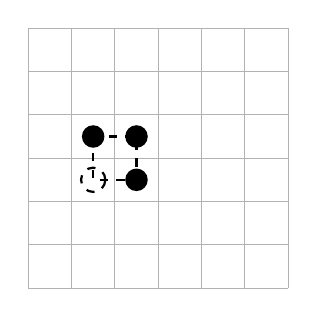
\begin{tikzpicture}[scale=0.55]
  \draw[gray!60] (0,0) grid (6,-6);
  \foreach \r/\c in {2/2, 3/2, 2/1}
    \fill[black] (\c+0.5,-\r-0.5) circle (0.26);
  \draw[thick,dashed] (1.5,-2.5) rectangle (2.5,-3.5);
  \draw[thick,dashed] (1.5,-3.5) circle (0.28);
\end{tikzpicture}
\caption{After the opening $(2,2)$, a far first reply, the second move
$(3,2)$, and the plan move $(2,1)$, the strategy (black) holds three corners
of the dashed block; the opponent must take the dashed cell $(3,1)$ or
lose on the next move.}
\label{fig:forcing}
\end{figure}

The plan above runs to completion against an opponent who always
blocks. On $\Board_6$ the line is
\[
  (2,2),\ (0,0),\ (3,2),\ (4,4),\ (2,1),\ (3,1),\ (1,1),\ (1,2),\ (1,0),
\]
\[
  (2,0),\ (2,3),\ (3,3),\ (0,3),\ (0,1),\ (2,5),\ (0,5),\ (4,3),
\]
first- and second-player moves alternating; every second-player move
is the unique block, and the last move threatens at both $(4,1)$ and
$(4,5)$, so one block leaves the other and reflex~(1) completes.
Figure~\ref{fig:line} shows the final position.

\begin{figure}[ht]
\centering
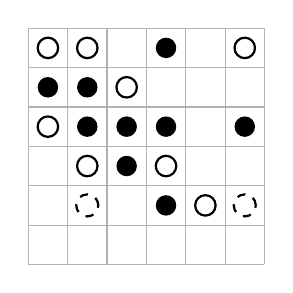
\begin{tikzpicture}[scale=0.5]
  \draw[gray!60] (0,0) grid (6,-6);
  \foreach \r/\c in {2/2, 3/2, 2/1, 1/1, 1/0, 2/3, 0/3, 2/5, 4/3}
    \fill[black] (\c+0.5,-\r-0.5) circle (0.26);
  \foreach \r/\c in {0/0, 4/4, 3/1, 1/2, 2/0, 3/3, 0/1, 0/5}
    \draw[thick] (\c+0.5,-\r-0.5) circle (0.26);
  \draw[thick,dashed] (1.5,-4.5) circle (0.28);
  \draw[thick,dashed] (5.5,-4.5) circle (0.28);
\end{tikzpicture}
\caption{The end of the displayed line. The strategy (black) threatens
at both dashed cells through the squares $\Sq(2,1,2)$ and
$\Sq(2,3,2)$; no single block answers both.}
\label{fig:line}
\end{figure}

Two features let one table serve every board of size at least six.
First, every cell a plan
can play lies in the corner region $\{0,\dots,5\}^2$, so each square
the strategy builds exists on every board with $n \ge 6$; this
confinement is a checked property of the table. Second, replies
outside the region are looked up through \emph{alignment classes}: a
far reply in row $r < 6$ falls in class $(\mathrm{row},\, r)$, one in
column $c < 6$ in class $(\mathrm{col},\, c)$, and the rest in a
default class. The classes reflect the geometry of
Lemma~\ref{lem:span}: every corner of a square through two stones of
the corner region lies in one of the region's rows or columns, so only
far replies aligned with the region can complete a square the strategy
is building. Third, a pair of far replies and a single region cell can be
three corners of one square; each branch carries entries keyed by
that cell, the pair's \emph{latent corner}
(Definition~\ref{def:latent}), storing plans that never surrender
it. When the first reply is not an exact key, the pair's latent
entry precedes the exact entry for $o_2$: exact entries answer the
generated board's geometry, which one far stone shifts.

The corner region is as small as a forcing table allows. A plan
confined to a $5 \times 5$ region has, on any board, exactly the
moves and squares it has on $\Board_5$, and faces there every reply
it faces inside the region on a larger board; a purely forcing
$5$-region table would therefore be a purely forcing strategy on
$\Board_5$, and the search reported below found none from the opening
$(2,2)$ over the second moves it considered.

The board of size $5$ is treated separately, and necessarily so: its
table is not purely forcing. Exhaustive analysis shows that for
twenty of the $(o_1, o_2)$ openings that arise, no all-forcing
continuation wins on $\Board_5$. The $5 \times 5$ table therefore
contains \emph{quiet forks}, a non-threatening move together with a
sub-table indexed by the reply to it, extracted from a full solution
of the $5 \times 5$ game: $1.79 \times 10^8$ positions solved, a
position being a pair of stone sets with the side to move, draws
scored against the first player. The solver reports the count when
it regenerates the table.

\subsection{The move function}
The layers combine into one procedure, stated in
Algorithm~\ref{alg:move} as it is defined in the formal development
(Section~\ref{sec:lean}). Lookups fall back from exact keys to
alignment classes to the default; the latent key of the reply pair,
when the pair has one, is taken before the exact key for $o_2$ if
$o_1$ has no exact key, and after it otherwise.

\begin{algorithm}[ht]
\caption{The move function.}\label{alg:move}
\begin{algorithmic}[1]
\If{some cell completes one of our squares}
  \State play the least such cell
\ElsIf{some cell completes an opponent square}
  \State play the least such cell
\ElsIf{we have not yet moved}
  \State play $(2,2)$
\ElsIf{we do not hold the tabled second move for $o_1$}
  \State play it
\Else
  \State select the entry by $(o_1, o_2)$; play the first plan cell
    we do not hold, and at a quiet fork play its move, then recurse
    on the sub-entry selected by the reply
\EndIf
\end{algorithmic}
\end{algorithm}

The general table holds $237$ branch keys (the $224$ possible first
replies on the board it was generated on, $\Board_{15}$, twelve
alignment classes, and a default) with $8{,}135$ plan entries and
$248$ latent entries in all; the $5 \times 5$ table holds $24$
branches. The generation board was raised until the table survived
the verification ladder: the table generated on $\Board_{13}$ is
refuted at $n = 14$, and the one generated on $\Board_{15}$ passes
every size up to $17$. The proof of Section~\ref{sec:uniform}
consumes the size only through the bound it puts on exact keys, which
keeps the anchor stones at coordinates $16$ and $17$ clear of them.
Both tables are included with the supplementary material in source
and machine-readable form.

\section{Verification}\label{sec:verify}

Fix a strategy $\sigma$ and a board size $n$. The
\emph{verification tree} of $\sigma$ on $\Board_n$ is the game tree
in which the first player's moves are given by $\sigma$ and the
second player's moves range over all empty cells; $\sigma$
\emph{verifies} on $\Board_n$ if every branch ends in a first-player
square.

\begin{proposition}\label{prop:verify}
If $\sigma$ verifies on $\Board_n$, then the first player wins the
square achievement game on $\Board_n$.
\end{proposition}

The $5 \times 5$ table is verified by a checker that walks this
tree in full; its soundness is the theorem \texttt{check\_sound} of
Section~\ref{sec:lean}. The forcing table is verified on a smaller
tree. The \emph{forced tree} of $\sigma$ on $\Board_n$ enumerates
the two reply levels in full and, below every later node, keeps only
the replies that block a threat of the move just played.

\begin{proposition}\label{prop:forced}
Suppose that past the second reply, at every node of the forced
tree, the strategy's move wins outright or leaves a threat, every
non-winning move and every threat cell lies in $\Board_6$, and no
empty cell completes an opponent square. If every branch of the
forced tree ends in a first-player square, then the first player
wins on $\Board_n$.
\end{proposition}

\begin{proof}[Proof sketch]
A reply blocking no threat leaves one standing, and the strategy
completes it on the next move, so every omitted reply loses in two
plies; the remaining obligations are those of
Proposition~\ref{prop:verify}. The formal statement is
\texttt{checkForced\_sound}.
\end{proof}

The forcing table satisfies these hypotheses for every
$6 \le n \le 17$ (Table~\ref{tab:runs}); with the $5 \times 5$ run,
the refutations of Section~\ref{sec:small}, and
Theorem~\ref{thm:uniform}, this proves Theorem~\ref{thm:main}. The
guards beyond winning are exactly the hypotheses
Section~\ref{sec:uniform} consumes.

\begin{table}[ht]
\centering
\begin{tabular}{rrcrr}
\toprule
$n$ & time (s) & & $n$ & time (s) \\
\midrule
5 & 1.5 & & 12 & 30 \\
6 & 0.2 & & 13 & 54 \\
7 & 0.6 & & 14 & 93 \\
8 & 1.5 & & 15 & 150 \\
9 & 3.6 & & 16 & 247 \\
10 & 7.7 & & 17 & 378 \\
11 & 16 & & & \\
\bottomrule
\end{tabular}
\medskip
\caption{Verification runs: wall-clock times of the compiled Lean
checkers on a laptop. The $5 \times 5$ run walks the full tree; the
others walk the forced skeleton. Each run is discharged by native
evaluation inside the ordinary build of the development.}
\label{tab:runs}
\end{table}

The search was implemented three times independently: a reference
implementation in Python used while discovering the tables, the formal
checker in Lean, and a TypeScript replay driving the interactive page
that accompanies the paper. All three return the same verdict on
every board size tested, and the TypeScript replay is additionally
checked move for move against exhaustive replays of whole boards and
of individual branches. A soundness theorem is proved for the Lean
checkers alone, and only their runs enter the proof of
Theorem~\ref{thm:main}.

\section{Formalization}\label{sec:lean}

The Lean development defines cells in the quarter-plane, boards as
finite subsets, squares as in Section~\ref{sec:defs}, and the winning
predicate as an inductive family: the first player \emph{can win} from
a position if some legal move completes one of their squares, or some
legal move admits at least one reply and every reply both fails to
complete an opponent square and leads to a position from which the
first player can win. A derivation of the predicate is precisely a
strategy tree, one first-player move per node with all replies
covered, and draws are failures by construction. These definitions,
a few dozen lines, are the whole specification: a reader audits them
by eye, and everything else is proved against them.

\begin{remark}\label{rem:terminal}
The predicate is read on positions reachable from the empty board,
where a game ends at its first square. On a position in which a
player already holds a square it does not say ``the game is over'':
a mover holding a square with no empty cell left cannot win in the
predicate's sense, since every constructor demands a move. Encoding
the end of the game explicitly would cost an extra hypothesis on
every constructor and every soundness proof, and buy nothing at the
empty board, so we keep the lean form and prove the outcome theorems
there. The one place the convention shows is
Lemma~\ref{lem:stealing}: the monotonicity step returns a disjunction,
a win or a completed square, exactly because the surplus stone may
end the game.
\end{remark}

The second player's win, and each player's ability to secure at least
a draw, are defined from the same predicate by swapping roles after a
move; a derivation of the draw predicate is a strategy tree whose
branches end in a win for its owner or a full board. Strategy
stealing and determinacy are proved against these definitions with no
computation, so the outcome theorem inherits its axioms from the
searches alone.

Three executable checkers are proved sound against this
semantics: \texttt{check}, which replays a strategy table against
all reply sequences, with
\[
  \texttt{check\_sound} \;:\;
  \texttt{check}\ t\ n = \texttt{true}
  \;\longrightarrow\; \text{the first player can win on } \Board_n;
\]
\texttt{checkForced}, which walks the forced skeleton of
Section~\ref{sec:verify} under its guards, with
\texttt{checkForced\_sound} of the same shape; and \texttt{refute},
the dual search of Section~\ref{sec:small}, with
\[
  \texttt{refute\_sound} \;:\;
  \texttt{refute}\ n = \texttt{true}
  \;\longrightarrow\; \text{the first player cannot win on } \Board_n.
\]
The move function that \texttt{check} replays, reflexes, the lookup
chain with its exact, latent, class, and default keys, and plan
resolution, is itself a Lean definition; Section~\ref{sec:strategy}
describes it, but the theorems depend only on the code.

The soundness proofs are short for the same reason: each checker
validates every move it plays. Legality is enforced by guards, completions are
detected by an executable scan proved equivalent to the abstract
predicate, and replies are enumerated exhaustively. Each proof is an
induction over the checker's recursion, and at every node the guards
supply exactly the premises of the corresponding constructor of the
winning predicate. Soundness
therefore never inspects the strategy; any table surviving the
guards yields a winning derivation, and the tables enter the
development purely as data. For the forced checker one further
ingredient appears: the two-move win against a non-blocking reply is
built by the soundness proof itself, once, instead of being searched
at every node. The recursion of each checker descends on an explicit
bound, $n^2 + 1$, on the number of moves in a game; exhausting the
bound returns failure, so the bound can cost completeness of the
search, never soundness of the theorem.

Concrete board sizes are discharged by native evaluation
(\texttt{native\_decide}): the statement that the first player can
win on $\Board_5$ is \texttt{check\_sound} applied to one evaluated
run of \texttt{check}, and each run of Table~\ref{tab:runs} is
discharged the same way. The axiom footprint of these theorems
is \texttt{propext}, \texttt{Classical.choice}, \texttt{Quot.sound},
and one instance of Lean's evaluation axiom for compiled reduction
per evaluated certificate. That last item is a genuine addition to
the trust base: the kernel checks the soundness theorems but not the
evaluations, which are performed by the Lean compiler and runtime.
Kernel reduction of the same runs is out of reach by orders of
magnitude, and a proof term recording every node of the search would
be larger than the tables by a similar factor, so we accept the
standard trust base of large computer-assisted proofs in Lean, and
report it.

\section{Every larger board}\label{sec:uniform}

\begin{theorem}\label{thm:uniform}
For every $n \ge 17$ the first player wins the square achievement
game on $\Board_n$. The winning strategy is constructed from the
forcing table: it replays the table's play from the checked run on
$\Board_{17}$, reading replies beyond that board through fixed
representatives.
\end{theorem}

The formal statement, \texttt{check\_sound\_uniform}, consumes
decidable hypotheses on a table: box size $6$, confined plans, one
forced-tree run on $\Board_{17}$, three families of anchored runs
described below, and a non-degeneracy condition on the second-move
map. The published table satisfies each by evaluation, in seconds.
The geometry rests on one containment.

\begin{lemma}\label{lem:span}
Let $x \ne y$ be distinct corners of a square $\Sq(r,c,s)$ with
$x, y \in \Board_B$. Then $r + s < 2B$ and $c + s < 2B$, so
$\Sq(r,c,s) \subseteq \Board_{2B}$; moreover every corner of
$\Sq(r,c,s)$ has its row or its column indexed below $B$.
\end{lemma}

\begin{proof}
Two distinct corners either share a coordinate and differ by $s$ in
the other, or differ by $s$ in both; either way $s < B$. Each anchor
coordinate is bounded by the corresponding coordinate of a corner, so
$r, c < B$, and the containment follows. For the last claim: if $x$
and $y$ share a row, the two remaining corners inherit their columns,
both below $B$; a shared column is symmetric; and if $x$ and $y$ are
diagonally opposite, all four corners lie in $\Board_B$.
\end{proof}

The constant $2B$ matches the development, which classifies a stone
as far exactly when one of its coordinates reaches $2B$; the bound
itself is not tight. A diagonal pair of corners confines the square
to $\Board_B$, and a same-row or same-column pair reaches coordinate
$2B - 2$ at most, attained by $\Sq(B-1, 0, B-1)$, so the tight
envelope is $\Board_{2B-1}$. A stone in the remaining ring is inert
by the same argument; the development counts it as near and resolves
it through exact entries, which loses nothing.

\begin{figure}[ht]
\centering
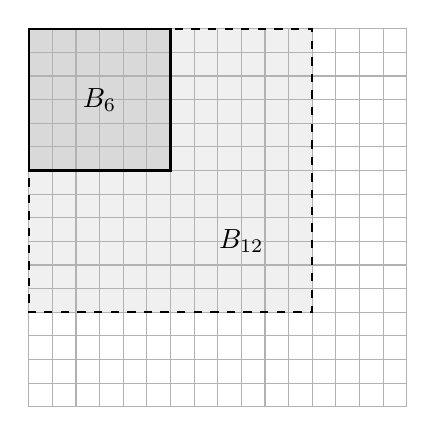
\begin{tikzpicture}[scale=0.3]
  \fill[gray!12] (0,0) rectangle (12,-12);
  \fill[gray!30] (0,0) rectangle (6,-6);
  \draw[gray!60] (0,0) grid (16,-16);
  \draw[thick] (0,0) rectangle (6,-6);
  \draw[thick,dashed] (0,0) rectangle (12,-12);
  \node at (3,-3) {$\Board_6$};
  \node at (9,-9) {$\Board_{12}$};
\end{tikzpicture}
\caption{The regions of the argument, drawn on $\Board_{16}$. Plans
stay in $\Board_6$; by Lemma~\ref{lem:span} every square through two
stones of $\Board_6$ lies in $\Board_{12}$; a stone beyond
$\Board_{12}$ shares no square with two near stones and meets the
play only through the classes and the latent entries.}
\label{fig:zones}
\end{figure}

In a position the forced run can reach, the opponent's lasting
stones are the two replies and forced blocks, and the guards of
Proposition~\ref{prop:forced} confine the blocks to $\Board_6$. An
opponent square therefore stands on a region cell, the two replies,
and the completing move.

\begin{definition}\label{def:latent}
A square is \emph{latent} for a pair of cells if both cells are
among its corners, a third corner lies in $\Board_6$, and the square
is not contained in $\Board_{17}$. The region corner is the pair's
\emph{latent corner}.
\end{definition}

\begin{lemma}\label{lem:dichotomy}
Let $\Sq(r,c,s)$ be latent for $\{x, y\}$, with region corner $b$
and $b, x, y$ distinct. Then $b = (r,c)$, $s \ge 12$, each of $x, y$
has a coordinate at least $12$, and $b$ depends only on $\{x, y\}$:
two squares latent for the same pair have the same latent corner.
\end{lemma}

\begin{proof}[Proof sketch]
Two corners in $\Board_6$ put the square inside $\Board_{11}$ by
Lemma~\ref{lem:span}, against escape; so $b$ is alone in the region,
and the corner positions force it northwest with $s \ge 12$. Each of
the three placements of $\{x, y\}$ on the remaining corners pins
$b$: an aligned member fixes a coordinate and the side, a diagonal
pair fixes both coordinates. The formal statement is
\texttt{escape\_farm}.
\end{proof}

\begin{remark}
The base $17 = 6 + 2 \cdot 6 - 1$ in Definition~\ref{def:latent} is
least. With base $15$, the replies $(0,16)$ and $(11,5)$ span a
square through the region cell $(0,5)$ completing at $(11,16)$: it
fits no board of size $15$, and $(11,5)$ has no coordinate at
$12$, so neither escape route of the dichotomy applies.
\end{remark}

\begin{lemma}[anchored safety]\label{lem:anchors}
For every region cell and every shape of pair admitting a latent
square with that corner (both members far; a region-aligned near
first member with a far partner; the mirror), the strategy, replayed
on $\Board_{23}$ from a concrete such pair under the guards of
Proposition~\ref{prop:forced}, never offers the corner as the unique
block. The runs range over coordinates rather than table keys,
finitely many in all, and each passes by evaluation.
\end{lemma}

The anchor pairs place one stone at coordinate $17$, just past the
base board, and the default-class anchor for the region cell $(a,b)$
puts its partner in row $a + 17 - b \le 22$; $\Board_{23}$ is the
least board holding every anchor. Any larger board would serve, since
the simulation transports a run from any base of size at least $17$;
the size only bounds the fuel and the square scan of the runs.

Figure~\ref{fig:farm} shows a latent square realized in play,
against an earlier table without latent entries.

\begin{proof}[Proof of Theorem~\ref{thm:uniform}, sketch]
Replay the checked run of $\Board_{17}$ on $\Board_n$. Replies on
the base board follow the checked tree verbatim; a reply that blocks
no standing threat loses to the threat at once; and the two reply
stones, when they leave the base board, are abstracted, through
stand-in cells when the pair has no latent corner and through the
runs of Lemma~\ref{lem:anchors} when it does, a block on the latent
corner itself being answered by the standing second threat. The
safety obligation at every node reduces to
Lemma~\ref{lem:dichotomy}: an opponent square is either inside
$\Board_{17}$ and excluded by the base run, or latent with a corner
the opponent never holds. The formal proof is \texttt{simulate} and
\texttt{check\_sound\_uniform}.
\end{proof}

\begin{figure}[ht]
\centering
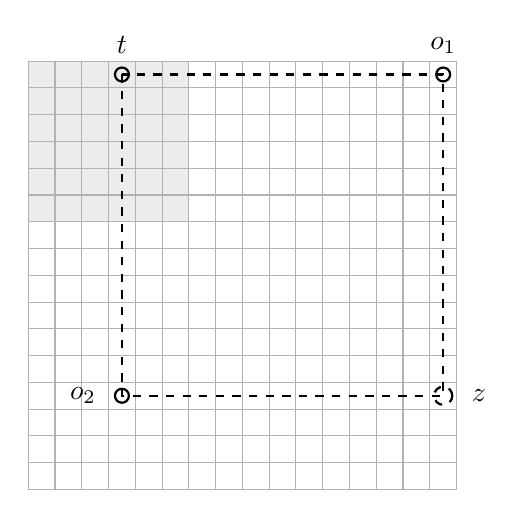
\begin{tikzpicture}[scale=0.34]
  \fill[gray!15] (0,0) rectangle (6,-6);
  \draw[gray!60] (0,0) grid (16,-16);
  \draw[thick,dashed] (3.5,-0.5) rectangle (15.5,-12.5);
  \foreach \r/\c in {0/3, 0/15, 12/3}
    \draw[thick] (\c+0.5,-\r-0.5) circle (0.26);
  \draw[thick,dashed] (15.5,-12.5) circle (0.34);
  \node[above=1pt] at (3.5,-0.2) {$t$};
  \node[above=1pt] at (15.5,-0.2) {$o_1$};
  \node[left=2pt] at (3.1,-12.5) {$o_2$};
  \node[right=2pt] at (16.0,-12.5) {$z$};
\end{tikzpicture}
\caption{A latent square on $\Board_{16}$, realized against an
earlier table without latent entries. The opponent's (white) free
replies $(0,15)$ and $(12,3)$ align with the corner region (shaded);
when a forced block lands on the region corner $t = (0,3)$, the
dashed square threatens at $z = (12,15)$. Two of its corners lie
outside $\Board_{15}$, so no search on that board encounters it.}
\label{fig:farm}
\end{figure}

\section{Reproducibility}\label{sec:repro}

The supplementary material contains the Lean development, with the
tables as data and each theorem above as a named declaration:
Theorem~\ref{thm:main} is \texttt{outcome}, whose first half is
\texttt{p1\_wins\_iff}; Lemma~\ref{lem:stealing} is
\texttt{second\_player\_no\_win}; Proposition~\ref{prop:small} is
\texttt{small\_board\_no\_win} with \texttt{small\_board\_drawn};
Theorem~\ref{thm:uniform} is \texttt{check\_sound\_uniform}; and the
supporting layer comprises \texttt{check\_sound},
\texttt{checkForced\_sound}, \texttt{refute\_sound},
\texttt{escape\_farm}, \texttt{simulate}, and the evaluated
certificates of Sections~\ref{sec:verify} and~\ref{sec:uniform}. The
development builds with no unproved declarations. Alongside it sit
the generation pipeline (strategy search, extraction, and export),
the reference verifier, and the commands that reproduce the runs of
Table~\ref{tab:runs} and the position count of
Section~\ref{sec:strategy}. The three copies of the tables, Lean
data, the page's JSON, and the pipeline's own, are regenerated from
the search and compared byte for byte in continuous integration, so
the checkers judge one and the same strategy. The interactive page
accompanying the paper replays the same tables move for move.

\section{Open questions}\label{sec:open}

The strategy is explicit but not short: $237$ branches and some eight
thousand plans. Is there a description of a winning strategy for all
$n \ge 6$ that a reader can carry in their head, in the style of
Jenrich's argument for $n = 5$ \cite{jenrich}, with no lookup table?
The confinement of the plans to a $6 \times 6$ region and the handful
of geometric cases in Section~\ref{sec:uniform} say that the winning
mechanism is local. In \cite{reid-plus} we give such a description: a
rule built on one shape, a stone with its four neighbours at a common
distance along the axes, prepared by at most three forcing moves, which
wins every board from $6$ up and is verified and formalized by the
same method as here.

The strategy is not optimal in length. The longest line in its
verified trees has $26$ plies on $\Board_6$, $\Board_7$, and
$\Board_8$, and $24$ plies for the separate table on $\Board_5$,
while the searches of \cite{adler} report a forced win within $13$
plies on every board from $6$ to $14$, one search per size, and the
rule of \cite{reid-plus} wins by the seventeenth ply on every board.
Is there a single strategy winning within $13$ plies on every board
from $6$ up? More generally, what is the least number of moves in which the
first player can force a win on $\Board_n$, and is there one strategy
that attains it for every $n$?

Are the constants least? The plan region cannot shrink below
$6 \times 6$ for a purely forcing table of this shape
(Section~\ref{sec:strategy}), and the base $17$ is least for the
dichotomy of Definition~\ref{def:latent}; the generation board $15$
is the smallest we found to work. Whether a finer abstraction of the
far replies lowers the base, or a different plan shape lowers the
region, is open.

\section*{Acknowledgements}

I thank Nicholas Tan for many games and for productive discussions
that shaped the strategy presented here.

\bibliographystyle{amsplain}
\bibliography{../shared/refs}

\end{document}
